\chapter{A Search For Truth}

Back in the day, certain doctrine was taught. Later on, those doctrines were
claimed to not have been transcribed correctly, meeting notes were questioned
and dismissed as not being current church doctrine.

Hard questions come up from time to time. We've been told to doubt our doubts.
Any questions that arise can be squashed with the spirit of the Lord as it were.
People are told to have faith. We don't have all the answers right now today,
but someday we will. Faith is needed.

It's a line. It's always just a line.

Then there are those few souls who understand and realize that questions can't
just easily be dismissed with faith. That it's okay to have questions. It's a
rare occurrence, and few indeed actually acknowledge this. Here are some
examples:

\begin{displayquote}
Gone are the days when a student asked an honest question and a teacher 
responded, ``Don't worry about it!" Gone are the days when a student raised a 
sincere concern and a teacher bore his or her testimony as a response intended 
to avoid the issue. Gone are the days when students were protected from people 
who attacked the Church. Fortunately, the Lord provided this timely and 
timeless counsel to you teachers: ``And as all have not faith, seek ye 
diligently and teach one another words of wisdom; yea, seek ye out of the best 
books words of wisdom; seek learning, even by study and also by 
faith."(Doctrine and Covenants 88:118)\footnote{The Opportunities and 
Responsibilities of CES Teachers in the 21st Century, 
Elder M. Russel Ballard, 2016}
\end{displayquote}

There is that famous quote by J. Rueben Clark:

\begin{displayquote}
If we have truth, [it] cannot be harmed by investigation. 
If we have not truth, it ought to be 
harmed.\cite{clark}
\end{displayquote}

\begin{figure}[h!]
  \centering
  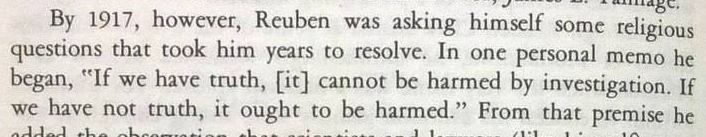
\includegraphics[width=0.4\linewidth]{articles/images/harm.png}
  \caption{J. Reuben Clark: The Church Years}
  \label{fig:clarkTruth}
\end{figure}

The quote should be cited in its full context of course. Because any and all 
sources should be found within their full context. Not only a portion. 
(See Appendix B: J. Reuben Clark: The Church Years)

Then there are the words of James E. Talmage:

\begin{displayquote}
The man who cannot listen to an argument which opposes his views either has a 
weak position or is a weak defender of it. No opinion that cannot stand 
discussion or criticism is worth holding. And it has been wisely said that the 
man who knows only half of any question is worse off than the man who knows 
nothing of it. He is not only one sided, but his partisanship soon turns him 
into an intolerant and a fanatic. In general it is true that nothing which 
cannot stand up under discussion and criticism is worth 
defending.\footnote{Editorial quoted in James E. Talmage, 
``Christianity Falsely So-Called," Improvement Era, Jan. 1920, 204.}
\end{displayquote}

George Albert Smith spoke on this very topic:

\begin{displayquote}
If a faith will not bear to be investigated; if its preachers and professors 
are afraid to have it examined, their foundation must be very 
weak.\footnote{George Albert Smith, Journal Of Discourses, v 14, page 216}
\end{displayquote}

Then M. Russell Ballard said the following counter claim:

\begin{displayquote}
We don't have to question anything in the church, don't get off into that. Just
stay in the Book of Mormon. Just stay in the Doctrine and Covenants. Just listen
to the prophets. Just listen to the apostles. We won't lead you astray, we
cannot lead you astray.\footnote{YSA Devotional, M. Russell Ballard, 2015}
\end{displayquote}

The church has released a handful of what they call Gospel Topic 
Essays.\footnote{https://www.lds.org/topics/essays?lang=eng} They are to shed
light on some of the history of the church that may or may not have been
widely known. This is a step in the right direction, however...it still feels
like the church is changing the narrative. Their history stated to the believers
has not always been the same. It has changed over time.

It is tempting to go through each of the essays...however I'm not sure I would
have the patience to go paragraph by paragraph and make notes on things found
and then look into the footnotes of each thing found.

Someday in the future I'm sure I will. There's no reason not to. If we are to
learn from the best books as it were, then the truth in those essays shouldn't
be scary. They should be welcomed with open arms. Is that possible in this day
and age of the internet? We have at our fingertips the ability to quickly search
for anything and everything. It could be considered dangerous.

I suppose, one needs to ask what is truth? If the truth can set you 
free,\footnote{John 8:32} then where exactly does the truth lay? Why is it so
difficult to find the truth at times? If the truth has been from the beginning
of the world, from before the beginning of the world, then it should be as
consistant as possible. It should be the same yesterday, today, tomorrow. All
truth should be the same and change shouldn't be a term in that narrative.

Yet the search for truth must go on.